\documentclass[12pt, letterpaper]{article}
\usepackage{graphicx}
\usepackage[top=1in, left=1in, right=1in, right=1in]{geometry}
\usepackage{float}

\begin{document}

\title{Devpi In The Cloud}
\author{Lee Hicks}

\maketitle

\section{What is this?}
This project is designing and implementing a Devpi server for pypi caching via Amazon Web Services (AWS).

\section{Versions}
There are multiple versions, all being a derivative of the base version.

\begin{itemize}
    \item Base - the bare minimum to get a devpi cache up in running via AWS 
    \item V1 - Base + Elastic Load Balancing (ELB) and AutoScaling
    \item V2 - V1 + Zenoss 
\end{itemize}

\section{Version - Base}
The base version is enough to deploy a devpi cache in AWS via CloudFormation (CF).

\subsection{Deployment}

\subsubsection{Required Files}
The necessary files for base deployment are located in the Project repo.

Important files:
\begin{itemize}
    \item Project/base/cf.json - CF script to bring up a single machine
    \item Project/base/puppet/devpi.pp - Puppet script used during instance provisioning
\end{itemize}

\subsubsection{Provisioning}
Ensure you have the required permissions to deploy instances, this also includes at least one set of EC2 KeyPair.

The setup is done in two parts, one is to host the Puppet configuration accessible to the EC2 instances. We will use
S3 to host the files. Once hosted we will update the cf.json script to point to that file and then use CF to bring
up the instance.

S3 steps:
\begin{enumerate}
    \item In S3 click Create Bucket and follow steps
    \item Once bucket is created, upload the devpi.pp file
    \item During upload set permissions to "everyone" so the instances can download the config
    \item Find the direct link for this S3 file, we will use that in the next section
\end{enumerate}

CF steps:
\begin{enumerate}
    \item Update the cf.json in the UserData section to curl the location above
    \item In CF click Create Stack and follow the instructions to create the stack
    \item On the Specify Parameters provide the URL for the puppet manifest.  
    \item On the Specify Parameters ensure "I acknowledge that this template may create IAM resources" is checked.  
    \item Once stack is created it will take at least 5 minutes for provisioning
\end{enumerate}

\subsubsection{Daily Operations}
There should be no daily operations associated with this setup.


\subsubsection{Architecture}
For a simple devpi server all that is needed is devpi. Devpi has a built in server via Bottle so with a few
commands devpi is installed and running. While the built in server is handy in my testing it seemed only to
serve requests that originate from localhost. The more permanent deployment is to put nginx in front of the
devpi cache.

\begin{figure}[H]
    \caption{Base Architecture}
    \centering
    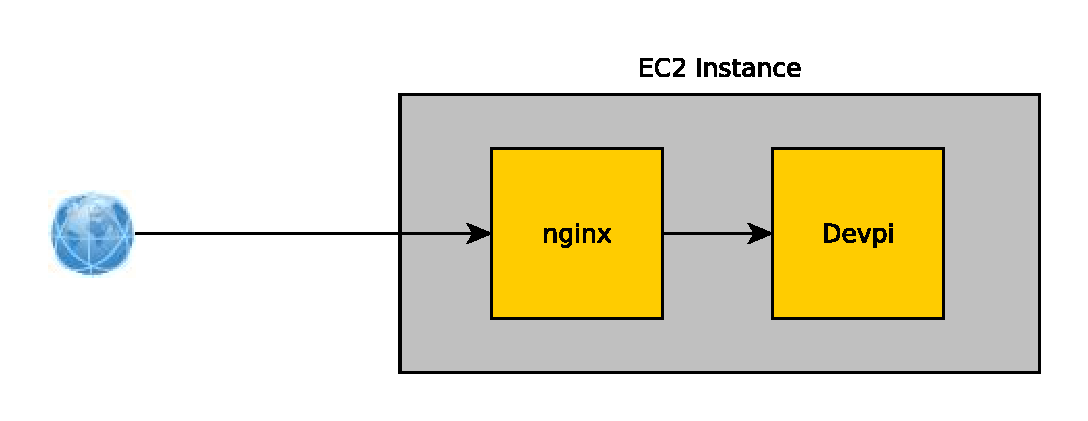
\includegraphics[width=\textwidth]{figures/base_arch.eps}
\end{figure}


\subsubsection{Implementation}
To deploy a simple devpi server a CF script was written. The CF script
is quite basic with starting a micro EC2 instance of Amazon Linux and applying the standard security policies of
port 22 and 80 open. CF Cloud-Init is used to install puppet. UserData fields was used to do some preparatory work before
puppet could be used. In this case the UserData field was used to fetch the initial puppet script and apply it.

\subsection{Puppet}
\subsubsection{How is it used?}
I debated quite a while on how I was going to use puppet for configuration. In the end I came to the conclusion that
running masterless puppet fit this application the best.  

The use case:
\begin{itemize}
    \item Security isn't a tight concern since these are pypi caches, not digitally signed
    \item The EC2 instances would be brought up and down at the drop of a hat
    \item They are only serving \textless 100 servers, no public cache
    \item Design to be near 100\% availability 
    \item Didn't need any reports
    \item I don't want to touch it once deployed, unless I have too... 
    \item Most importantly KISS
\end{itemize}

\subsubsection{Going Masterless}

Using a puppet master (PM) requires at least a dedicated EC2, if not more, to be on the safe side. This could be ran on an instance
that is also serving devpi. The only problem is when under load any extra processing seems to kill micro instance performance.
More importantly, a PM now becomes a single point of failure. If the PM goes down the replacement instance won't become a new PM,
without manual setup. Until the new PM can be installed and configured new instances can't receive the puppet manifest and will fail
to be configured. 

So to reduce that risk one could put a puppet master behind another ELB with dedicated instance, increasing cost, and also adding 
a whole host of new problems like master slave PMs, how do we enforce that, when the master goes down how does trust get 
transferred to slave PM, and does it scale? A rabbit whole of issues to solve that masterless puppet setup steers around.

\subsubsection{Implementation}

\begin{figure}[h]
    \caption{Detailed Deployment Process}
    \centering
    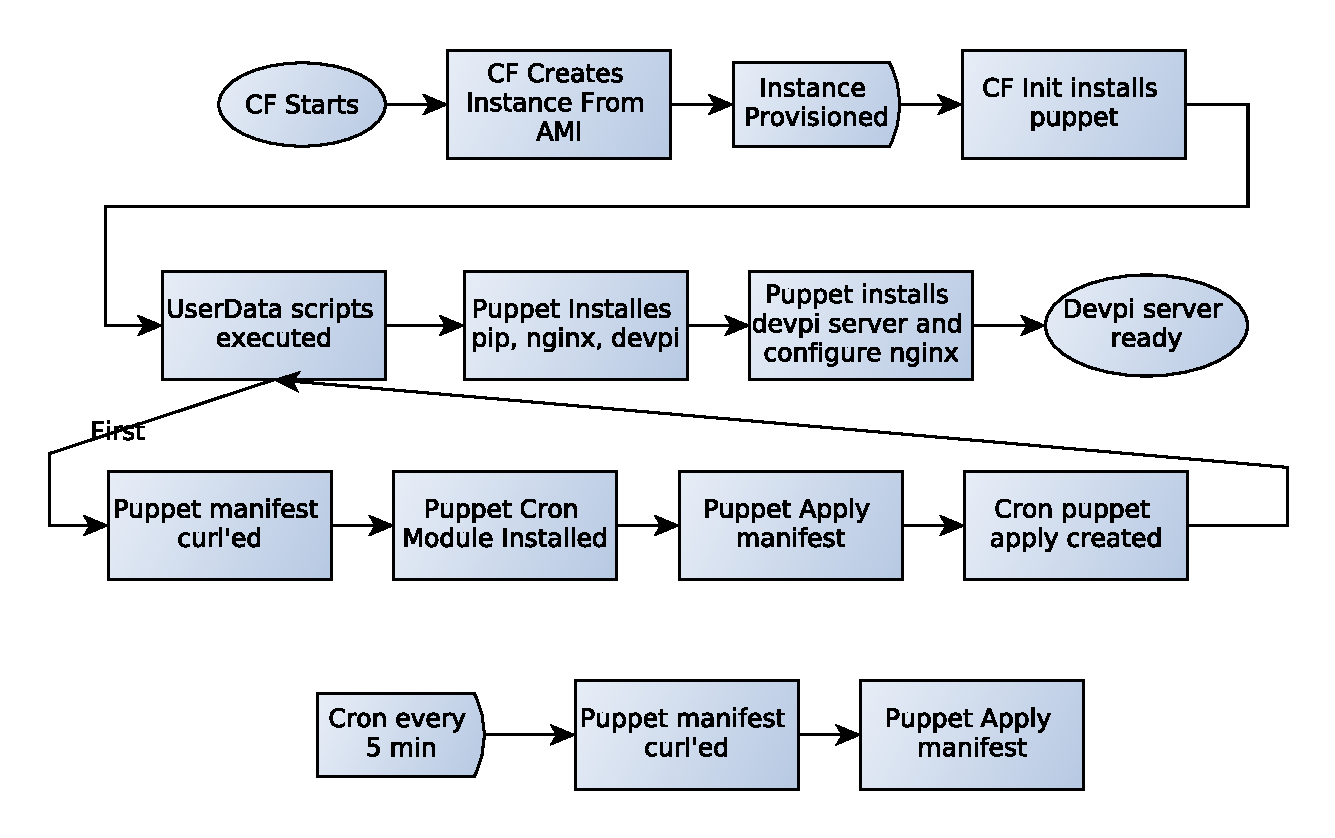
\includegraphics[width=\textwidth]{figures/base_setup.eps}
\end{figure}
\begin{enumerate}
    \item Puppet init stored on S3 bucked
    \item Instanced fired up via CF using CF-init and UserData script
    \item CF-init ensures puppet is installed
    \item Userdata script grabs the init .pp file and applies it
    \item Puppet applies the manifest and also creates a cron job to fetch and apply every X minutes (our case 30) 
\end{enumerate}

Since the cron jobs runs every X minutes, applying updates to manifest is as simple as uploading a new manifest to the S3 bucket.

This setup allows any AMI that is RHEL based, using yum, to use this process without requiring us to bake our own AMIs. This can
be extended very easily to any AMI that CF-init supports by switching the package manager.


\subsection{Analysis}
\subsubsection{Performance}
Stress testing was tested with siege. Siege simulates many GET requests, though this doesn't exactly align with devpi it is the only 
metric I could easily simulate. Simulating high pip usage against devpi would have been out of the scope of this project. It
would have required a single medium or larger EC2 instance for spawning pip instances and high bandwidth throughput, my ISP bandwidth
would not suffice.

Siege tests have been extremely erratic from 50 req/s to almost 200 req/s. Any higher, response time increases and 5XX errors become
the norm. While monitoring system resources devpi process never fully utilizes system resources, and once a 5XX code is generated 
devpi fails to recover. With this it might be plausible that something internal, queue/polling, to devpi is hurting performance.

A larger EC2 instance could mitigate poor performance, but this particular performance issues stems from software not hardware.

\subsubsection{Cost}
Cost calculation is simple for this setup. With a single instance running devpi falls in the AWS Free Usage Tier, S3 access every
5 minutes totals to 8640 request \textless 20K requests included in the free tier. This setup does not incur cost month to month.

\subsubsection{Woes/Drawbacks}
As mentioned above one of the drawbacks is using only built in puppet modules, if you need additional modules your on your own. 
Example of this is setting up the cron job. The tao of puppet is puppet defines the state the system should
be in rather than using rules and executing shell commands. Researched turned up little on how to instruct puppet to install modules
without a PM. To overcome this issue puppet modules is installed using shell scripts in the UserData section.

To complicate matters, puppet installs modules in several places, /etc/puppet/modules: /usr/share/puppet/modules. When 
/etc/puppet/modules wasn't found it would halt without trying other paths defined. As a quick fix in UserData the /usr/puppet/modules
directory is created.

Another issue is security, currently at the time of writing the manifest is on a public S3 bucket. For this usecase this isn't
an issue since no sensitive information is contained within the manifest. For more sensitive manifests it is possible to define 
permissions in CF script so each EC2 instance can read the manifest.

\subsection{Conclusion}
The best use case for this is to have a puppet configurable devpi cache that is always on, and possibly shared with a few devs. 

\section{Version - V1}

\subsection{Deployment}
Steps almost exactly like base version but here for reference.

\subsubsection{Required Files}
The necessary files for V1 deployment are located in the Project repo.

Important files:
\begin{itemize}
    \item Project/V1/cf.json - CF script to bring up a single machine
    \item Project/V1/puppet/devpi.pp - Puppet script used during instance provisioning
\end{itemize}

\subsubsection{Provisioning}
Ensure you have the required permissions to deploy instances, this also includes at least one set of EC2 KeyPair.

The setup is done in two parts, one is to host the Puppet configuration accessible to the EC2 instances. We will use
S3 to host the files. Once hosted we will update the cf.json script to point to that file and then use CF to bring
up the instance.

S3 steps:
\begin{enumerate}
    \item In S3 click Create Bucket and follow steps
    \item Once bucket is created, upload the devpi.pp file
    \item During upload set permissions to "everyone" so the instances can download the config
    \item Find the direct link for this S3 file, we will use that in the next section
\end{enumerate}

CF steps:
\begin{enumerate}
    \item Update the cf.json in the UserData section to curl the location above
    \item In CF click Create Stack and follow the instructions to create the stack
    \item On the Specify Parameters ensure provide the URL for the puppet manifest  
    \item On the Specify Parameters ensure "I acknowledge that this template may create IAM resources" is checked
    \item Once stack is created it will take at least 5 minutes for provisioning
\end{enumerate}

\subsubsection{Daily Operations}
There should be no daily operations associated with this setup.

\subsubsection{Architecture}
Taking the base version and extending for high traffic and availability it was obvious that some type of redundancy was needed. 
Each instance is stand alone with no dependencies or shared resources, this makes it extremely easy to scale. AWS offers an 
ELB for distributing traffic. AWS also offers AutoScaling groups to manage high and low traffic spikes.

This design has a public facing ELB. Behind the ELB is an AutoScaling group that contains at least one devpi
server. The ELB will register instances that it determines is healthy, and start distributing traffic with the new instance.   

\begin{figure}[H]
    \caption{V1 Architecture}
    \centering
    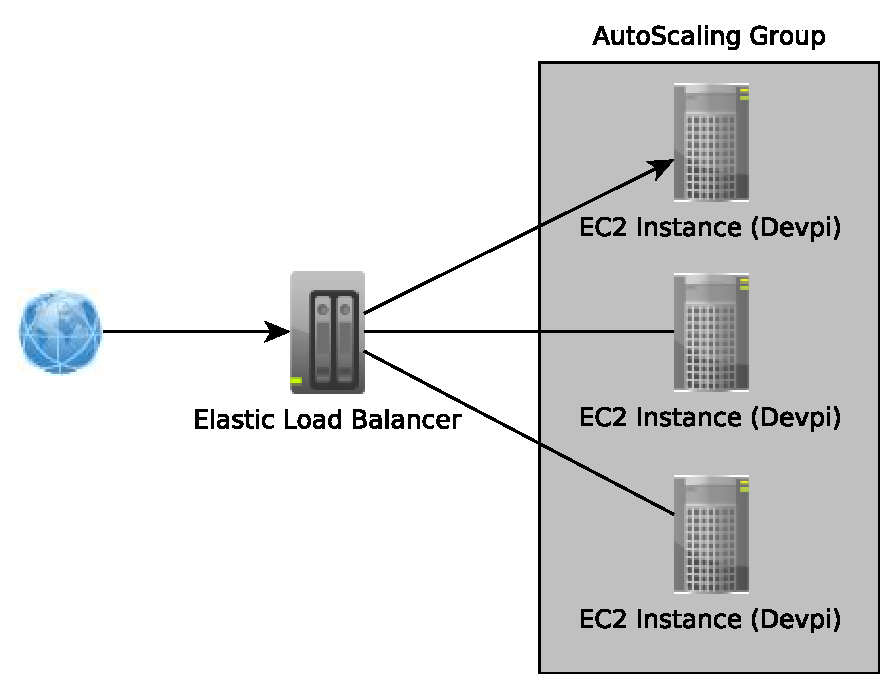
\includegraphics[width=0.75\textwidth]{figures/v1_arch.eps}
\end{figure}

\subsubsection{Implementation}
This AutoScaling cluster is entirely written in CF script and follows the same provisioning setup as the base, except in a cluster.

The ELB is setup together with AutoScaling. Alarms are set to monitor the ELB request latency and 5XX response codes.

\begin{itemize}
    \item Latency \textgreater 10s, observed for 1m will increase AutoScaling group by 1
    \item Latency \textless 5s, observed for 10m will decrease AutoScaling group by 1
    \item 5XX errors \textgreater 5, observed for 1m will increase AutoScaling group by 1
    \item 5XX errors $<=$ 0, observed for 5m will decrease AutoScaling group by 1
\end{itemize}

The alarms are more aggressive on high loads to expand quickly and shrink slowly as traffic wanes. The observation periods
include instance provisioning delay of ~90s for a devpi instance to come online. The ELB has health checks of 60s for healthy, and
2.5m for unhealthy. Even with hard set thresholds, the ELB can sometimes take much longer than expected to register instances 
to the load balancing pool.

\subsection{Puppet}
\subsubsection{How is it used?}
Puppet is used in the same fashion as base version. Since there is no puppet master one can provision hundreds of instances
with no bottleneck or single point of failure.

\subsection{Analysis}
\subsubsection{Performance}
Stress testing was tested with Siege. Again to reiterate that this is a horrible test for a pypi cache. The best test
results were with a cluster of four devpi instances processing 266 req/s, request latency \textless 0.15s, and no 5XX responses.
Your mileage will vary!

\subsubsection{Cost}
Cost calculations should only be taken with a grain of salt, because the usecase didn't provide traffic metrics such as
how many packages to be updated, how many servers will use devpi, the frequency of updates...etc. Below are two cost scenarios,
one is super light, a few requests a day for a couple of servers, the other is a sustained 100req/s. Each scenario is 
expandable with autoscaling and ELB already included in pricing.

Constants:
\begin{itemize}
    \item Each pip request reply is 500B (empirical average)
    \item Each pip package download is 500Kb
\end{itemize}

\begin{table}[H]
    \caption{Monthly cost at 2K requests per day, 10\% of requests result in package download}
\begin{center}
    \begin{tabular}{l c c c c}
        Service     & Instances & Scalar  & Cost/Unit & Sum     \\
        \hline
        EC2         & 1         & 720hr   & \$0.02    & \$14.40 \\
        ELB         & 1         & 720hr   & \$0.025   & \$18.00 \\
        ELB Traffic & .03       & 1gb     & \$0.008   & \$0.00  \\
        EBS         & 10        & 1gb/m   & \$0.10    & \$1.00  \\
        Cloudwatch  & 1         & 1/m     & \$3.50    & \$3.50  \\
        \hline
                    &           &         & Total     & \$36.90
    \end{tabular}
\end{center}
\end{table}

\begin{table}[H]
    \caption{Monthly cost at 100 requests per second, 0.1\% of requests result in package download}
\begin{center}
    \begin{tabular}{l c c c c}
        Service     & Instances & Scalar  & Cost/Unit & Sum     \\
        \hline
        EC2         & 2         & 720hr   & \$0.02    & \$28.80 \\
        ELB         & 1         & 720hr   & \$0.025   & \$18.00 \\
        ELB Traffic & 1.5      & 1gb     & \$0.008   & \$0.24  \\
        EBS         & 20        & 1gb/m   & \$0.10    & \$2.00  \\
        Cloudwatch  & 2         & 1/m     & \$3.50    & \$7.00  \\
        \hline
                    &           &         & Total     & \$55.92
    \end{tabular}
\end{center}
\end{table}


\subsubsection{Scalability/Availability}
Since the majority of the bottleneck is the devpi server itself, reducing traffic to devpi instances itself would benefit with less
5XX errors, server crashing, and lower monthly cost since less instances would have to be ran. A caching proxy/reverse proxy in front
of the instances would greatly benefit response time and offload much work from devpi service to the proxy cache.

A reverse proxy called Varnish seems ideal for this setup. Varnish stored the cached items in RAM for improved performance. Because
of this an EC2 instance larger than micro would be needed, more RAM the better. Varnish supports both HTTP and file caching meaning
Varnish could respond to pip requests and serve pypi packages, if cached, itself without passing the request to devpi instance. If items
aren't stored in the cache the request is proxied to a devpi instance, served, then cached for future requests. 

An issue with caches is how does the cache keep in sync with the content it is caching? Varnish allows purging of cached objects via through
Varnish commands or HTTP requests. The simplest purging setup is to have a cron job run every X hours to purge the entire cache. Requests coming 
in will fill the cache up over time. Uncached items will have a single penalty with the request being passed to the devpi instance.

A more complicated method is to have devpi notify varnish that a cached object needs to be purged, new pypi package became available. This
will probably take modification of the devpi server so it can update its cache. This then becomes the issue of caching a cache.

In the past AWS has had issues with a region going down. To overcome this possible outage and provide redundancy utilizing AWS Route53
service can help. Route53 has a DNS failover feature that can detect when a primary application is down, similar to the health checks used
by ELB in determining instance states. Route53 will automatically remove a region and forward all traffic to a backup region. This does
require to have a minimum of  at least two clusters, one in each region, that will increase monthly costs. These costs can be offset by 
providing geographical optimizations if users are international, for this usecase both regions should be located in US.

\subsubsection{Woes/Drawbacks}
Care must be taken when determining thresholds, with the current threshold there is a buffer for winding up or down instances. This
is to reduce a flux of the AutoScaling group. These buffer threshold may need to be tweaked a little better than what they are
currently set at.

Another issue that was encountered was the ELB taking a while to register instances. Most of the time long registration times is
to be blamed on unhealthy checks taking place while puppet is still applying the manifest. When puppet is complete, the ELB has 
already marked the instance as unhealthy, and healthy checks must take place before ELB registration is done. This hiccup 
normally happens at the worst possible time because the AutoScaling group is growing due to load. If the ELB takes too long to 
register the AutoScaling group will cool down and add another devpi instance before the first devpi instance has been registered.  

\subsection{Conclusion}
The best use case for this design is a deployment of servers that requires high availability cache.

\end{document}
